% ==================///==================///==================///
% ==================/// LATEX'S STUFF
% ==================///==================///==================///

\documentclass{beamer}
\usepackage{amsfonts,amsmath,oldgerm}
\usepackage{listings}
\usepackage{colortbl}
\usetheme{_statale}
\usefonttheme[onlymath]{serif}


\setbeamertemplate{caption}[numbered]
\newcommand{\testcolor}[1]{\colorbox{#1}{\textcolor{#1}{test}}~\texttt{#1}}
\newcommand{\hrefcol}[2]{\textcolor{frmtxt}{\href{#1}{#2}}}
\titlebackground*{assets/background}

% ==================///==================///==================///
% ==================/// SPLASH PAGE
% ==================///==================///==================///

\title{Why study Topology?}
\subtitle{Pointset Topology}
\course{Topology Summer Camp}
\author{AZZEDDINE Yacine}
\IDnumber{yacine.azzeddine@nhsm.edu.dz}
\date{20th of July, 2025}

% ==================///==================///==================///
% ==================/// START PRESENTATION
% ==================///==================///==================///

\pgfplotsset{compat=1.18}
\usetikzlibrary{positioning}
\begin{document}
\maketitle

% ==================///==================///==================///
% ==================/// BODY'S PRESENTATION
% ==================///==================///==================///
\section{The Summer Camp's Format}
\begin{frame}
    \frametitle{How will the summer camp function?}

    \begin{itemize}
        \item Almost every week there will be a 1-1.5h lecture wherein you are expected to attend
        \pause
        \item There will be a weekly homework of varying difficulty. Each homework submission
        will be read and given feedback \pause
        \item Every now and then there will be held office hours \pause
    \end{itemize}
    I want to emphasize that the summer camp is NOT a substitute for self-studying
\end{frame}


\section{Motivation}

\begin{frame}<0>[label=motivation]
    \frametitle{Why do we study topology?}

    \begin{itemize}
        \item<1-> formalization of intuitive notions
        \item<2-> providing the right setting to study geometric objects (manifolds)
        \item<3-> standardizing notions 
        \item<4-> Careful treatment of infinite objects
    \end{itemize}

\end{frame}

\againframe<1>{motivation}

\begin{frame}[label=jordan]
    \frametitle{Formalization of Intuitive Notions}

    \begin{theorem}
        a non-self-intersecting closed curve on the plane (i.e. a jordan curve) divides the plane into
        two regions: a bounded interior and an unbounded exterior
    \end{theorem}
    \pause
    \begin{columns}
        \begin{column}{0.48\textwidth}
            \begin{block}{Jordan Curve}
                \vspace*{3cm}
            \end{block}
        \end{column}
        \begin{column}{0.48\textwidth}
            \begin{block}{not a Jordan Curve}
                \vspace{3cm}
            \end{block}
        \end{column}
    \end{columns}

\end{frame}

\begin{frame}
    \frametitle{Formalization of Intuitive Notions}

    \begin{proof}[proof of the jordan curve theorem]
        We shall use proof by f*cking obviousness. It's a closed loop. Of course there's going to be an outside and inside. 
        Humans have been making borders and fences for millennia and this still needs to be proven?"? What am I supposed to say?
        It's so bloody obvious! 
        It's like trying to prove 1+1=2. Why is this even a theorem? Not even worth to be a Lemma or Corollary tbh. 
        This trivial ass b*tch.
        And thus concludes the proof of the "theorem".
    \end{proof}

\end{frame}

\begin{frame}
    \frametitle{Formalization of Intuitiva Notions}

    \begin{theorem}[Jordan Curve Theorem]
        a non-self-intersecting closed curve on the plane (i.e. a jordan curve) divides the plane into
        two regions: a bounded interior and an unbounded exterior
    \end{theorem}

\end{frame}

\begin{frame}
    \frametitle{Formalization of Intuitiva Notions}

    \begin{theorem}[Jordan Curve Theorem (more formally)]
        suppose $C=\operatorname{Im} \phi$ where $\phi\colon [0, 1]\longrightarrow \bR^2$ such that $\phi$ is \alert{continuous}, 
        $\phi(0) = \phi(1)$ and $\phi_{|(0, 1)}$ is injective. Then $\bR^2\setminus C$ splits into two \alert{connected components}
        one of which is \alert{precompact} and the other is unbounded.
    \end{theorem}

\end{frame}

\againframe<2>{motivation}

\begin{frame}
    \frametitle{The Right Setting to Study Geometry}

    \begin{columns}
        \begin{column}{0.5\textwidth}
            Topology allows us to study the properties of geometric object that are preserved under continuous deformations, such as stretching, 
            twisting, crumpling, and bending; that is, without closing holes, opening holes, tearing, gluing, or passing through itself. 
        \end{column}
        \begin{column}{0.5\textwidth}
            \begin{block}{coffis cup}
                \href{https://upload.wikimedia.org/wikipedia/commons/2/26/Mug_and_Torus_morph.gif}{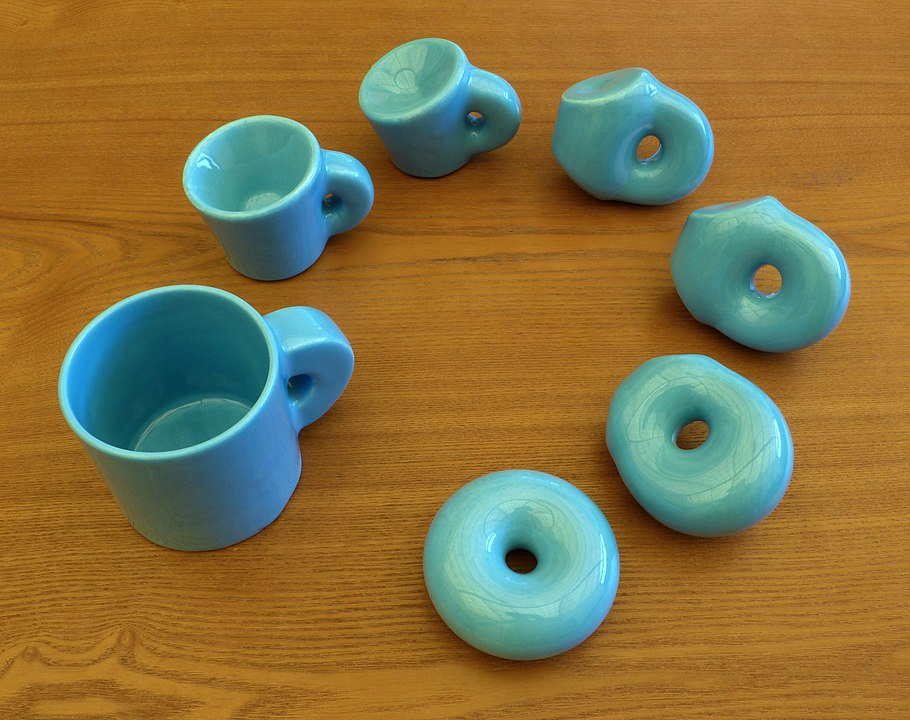
\includegraphics[width=\textwidth]{assets/mug_torus.jpg}}
            \end{block}
        \end{column}
    \end{columns}

\end{frame}

\begin{frame}
    \frametitle{The Right Setting to Study Geometry}

    \begin{block}{a cube is just a sphere}
        §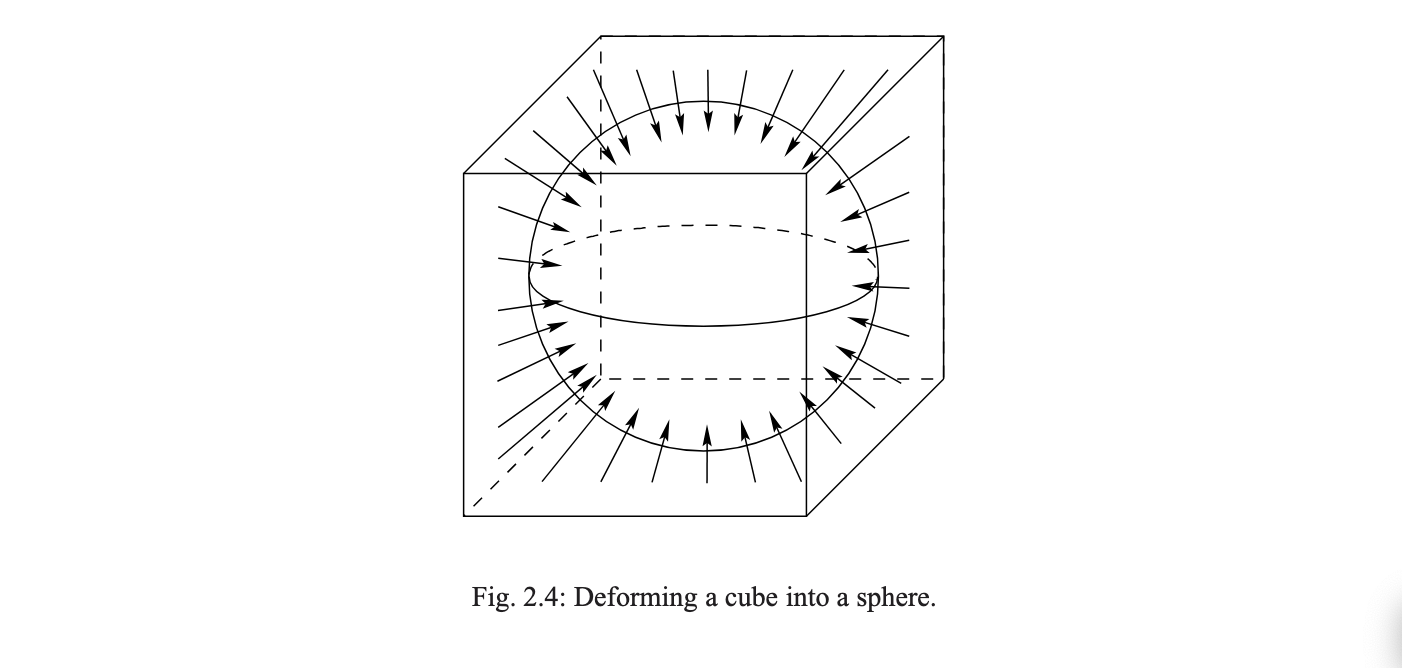
\includegraphics[width=\textwidth]{assets/cubetosphere.png}
    \end{block}

\end{frame}

\againframe<3>{motivation}

\begin{frame}
    \frametitle{Standardizing notions}

    \begin{itemize}
        \item In math, every notion has a couple million different ways to be defined. General topology standardizes all of that \pause
        \item Topology is a very convenient setting to encode information \pause
        \item The language used in studying topology is standard across all fields
    \end{itemize}

\end{frame}

\againframe<4>{motivation}
\begin{frame}
    \frametitle{careful treatment of infinite objects}

    \begin{theorem}[(false)]
        Let $f\colon A\longrightarrow \bR$ be a real function. There must exist an $x_0\in A$ such that for all $x\in A$
        \[f(x_0)\geq f(x)\]
    \end{theorem} \pause
    This theorem is obviously true if $A$ is a finite set. \pause Things get a lot more complicated if $A$ is infinite however. So you might ask, what 
    are the weakest assumptions can we add for the theorem to remain true? \pause Topology allows us to answer this.

\end{frame}

\section{Rediscovering the Definition}

\begin{frame}
    \frametitle{Spoilers!}

    \begin{definition}
        Let $X$ be any set. A topology on $X$ is a collection $\tau$ of subsets of $X$ that satisfy the following properties: \pause
        \begin{enumerate}
            \item $\varnothing, X\in \tau$
            \item $\tau$ is closed under arbitrary unions: if $I$ is an indexing sets and $(A_i)_{i\in I}\subset \tau$ then
            $\bigcup_{i\in I} A_i\in \tau$
            \item $\tau$ is closed under finite intersections: if $(A_i)_1^n$ is a finite collection of elements of $\tau$ then
            $\bigcap_{i=1}^n A_i\in\tau$
        \end{enumerate}\pause
        The couple $(X, \tau)$ is called a topological space and elements of $\tau$ are called open sets.
    \end{definition}

\end{frame}

\begin{frame}[label=continuity]
    \frametitle{Continuity}

    \textbf{our goal from this section is to rediscover the definition of topology}
    \pause

    We start our mission from a familiar definition of continuity: \pause
    \begin{definition}
        suppose $f\colon(a, b)\longrightarrow\bR$ is a function. We say that $f$ is continuous if $\forall x\in(a, b)$, $\forall\eps>0\exists\delta>0$ 
        such that:
        \[\abs{x-y}<\delta \implies \abs{f(x)-f(y)}<\eps\]
    \end{definition}
    
\end{frame}

\begin{frame}
    \frametitle{Continuity}

    \begin{block}{graph}
        \vspace{5cm}
    \end{block}

\end{frame}

\againframe<3>{continuity}

\begin{frame}
    \frametitle{metric spaces}

    The most important aspect of the previous definition is that we are given a method of calculating error. A \alert{metric} which
    measures the distance between two points $x$ and $y$: $d(x, y) = \abs{x-y}$ \pause That is to say, if we had any method of calculating
    distance we would be able to define continuity again! \pause For that reason we make the following definition
    \begin{definition}
        A \alert{metric space} is a tuple $(X, d)$ such that $d\colon X\times X\longrightarrow\bR^+$ is a function which satisfies
        \begin{enumerate}
            \item (positivity) $d(x, y) = 0$ iff $x=y$. Otherwise, $d(x, y)>0$
            \item (symmetry) $d(x, y) = d(y, x)$ $\forall x, y\in X$
            \item (triangle inequality) $\forall x, y, z\in X$
            \[d(x, z) \leq d(x, y) + d(y, z)\]
        \end{enumerate}
    \end{definition}

\end{frame}

\begin{frame}
    \frametitle{Example 1: The Real Line}
    \textbf{Metric:} $d(x, y) = |x - y|$ on $\mathbb{R}$
    \newline
    \textbf{Axioms:} \pause
    \begin{enumerate}
        \item \textbf{Non-negativity:} $|x-y| \geq 0$ and $|x-y| = 0 \iff x-y = 0 \iff x = y$ \pause
        \item \textbf{Symmetry:} $|x-y| = \abs{-(x-y)} = |y-x|$ \pause
        \item \textbf{Triangle inequality:} since we know $\abs{a+b}\leq\abs{a}+\abs{b}$
        \[|x-z| = \abs{(x-y)+(y-z)} \leq |x-y| + |y-z|\]
    \end{enumerate}
\end{frame}

\begin{frame}
    \frametitle{Example 2: Euclidean Space}
    \textbf{Metric:} $d(\mathbf{x}, \mathbf{y}) = \sqrt{\sum_{i=1}^n (x_i - y_i)^2}$ on $\mathbb{R}^n$\pause
    \newline
    \textbf{Axioms:}
    \begin{enumerate}
        \item \textbf{Non-negativity:} Each $(x_i - y_i)^2 \geq 0$, so $d(\mathbf{x}, \mathbf{y}) \geq 0$; $d(\mathbf{x}, \mathbf{y}) = 0 \iff \mathbf{x} = \mathbf{y}$ \pause
        \item \textbf{Symmetry:} $d(\mathbf{x}, \mathbf{y}) = d(\mathbf{y}, \mathbf{x})$\pause
        \item \textbf{Triangle inequality:} Left for homework
    \end{enumerate}
\end{frame}

\begin{frame}
    \frametitle{Example 3: Discrete Metric}
    \textbf{Metric:} take any set $X$ and let $d(x, y) = \begin{cases} 0 & x = y \\ 1 & x \neq y \end{cases}$\pause
    \newline
    \textbf{Axioms:}
    \begin{enumerate}
        \item \textbf{Non-negativity:} $d(x, y) \in \{0, 1\}$, and $d(x, y) = 0 \iff x = y$ \pause
        \item \textbf{Symmetry:} $d(x, y) = d(y, x)$\pause
        \item \textbf{Triangle inequality:} $d(x, z) \leq d(x, y) + d(y, z)$ (check all cases)
    \end{enumerate}
\end{frame}

\begin{frame}
    \frametitle{Example 4: Supremum Metric on $C([a, b])$}
    \textbf{Metric:} $d(f, g) = \sup_{x \in [a, b]} |f(x) - g(x)|$ for $f, g \in C([a, b])$ \pause
    \newline
    \textbf{Axioms:}
    \begin{enumerate}
        \item \textbf{Non-negativity:} $|f(x) - g(x)| \geq 0$, so $d(f, g) \geq 0$; $d(f, g) = 0 \iff f = g$ \pause
        \item \textbf{Symmetry:} $|f(x) - g(x)| = |g(x) - f(x)|$ Therefore, \[\sup_{x \in [a, b]} |f(x) - g(x)| = \sup_{x \in [a, b]} |g(x) - f(x)|\]
        which implies,
        \[d(f, g) = d(g, f)\]
    \end{enumerate}
\end{frame}

\begin{frame}
    \frametitle{Example 4: Supremum Metric on $C([a, b])$ (continued)}

    \begin{enumerate}
        \setcounter{enumi}{2}
        \item \textbf{Triangle inequality:} for all $x\in[a, b]$ we have 
        \begin{align*}
            |f(x) - h(x)| &\leq |f(x) - g(x)| + |g(x) - h(x)| \\
            &\leq d(f, g)+d(g, h)
        \end{align*}
        but that would mean
        \[\sup_{x \in [a, b]} |f(x) - h(x)| \leq d(f, g) + d(g, h)\]
        hence
        \[d(f, h) \leq d(f, g) + d(g, h)\] as required
    \end{enumerate}

\end{frame}

\begin{frame}
    \frametitle{continuity in metric spaces}

    Now that we have a let's what our definition of continuity would look like \pause
    \begin{definition}
        Let $(X, d)$ and $(Y, d')$ be two metric spaces and suppose $f\colon X\longrightarrow Y$ is a function. We say that $f$ is continuous if $\forall x\in X$, $\forall\eps>0\exists\delta>0$ 
        such that:
        \[d(x, y)<\delta \implies d'(f(x), f(y))<\eps\]
    \end{definition}

\end{frame}

\begin{frame}
    \frametitle{continuity in $\bR^n$}

    now that we have continuity defined we can use to define continuous function between, say, $\bR^n$ and $\bR$: \pause
    \begin{definition}
        Suppose $f\colon \bR^n\longrightarrow \bR$ is a function. We say that $f$ is continuous if $\forall x\in \bR^n$, $\forall\eps>0\exists\delta>0$ 
        such that:
        \[\norm{x-y}<\delta \implies |f(x), f(y)|<\eps\]
    \end{definition} \pause
    or, for example, $\bR$ and the discrete metric on $X$!
    \begin{definition}
        Suppose $f\colon \bR\longrightarrow X$ is a function. We say that $f$ is continuous if $\forall x\in \bR$, $\forall\eps>0\exists\delta>0$ 
        such that:
        \[\abs{x-y}<\delta \implies d(f(x), f(y))<\eps\]
    \end{definition} \pause
\end{frame}

\begin{frame}
    \frametitle{Some properties}

    \begin{theorem}
        if $f\colon (X, d_X)\longrightarrow(Y, d_Y)$ and $g\colon(Y, d_Y)\longrightarrow(Z, d_Z)$ are continuous function between 
        metric spaces then $g\circ f\colon(X, d_X)\longrightarrow(Z, d_Z)$ is also continuous
    \end{theorem} \pause
    \begin{theorem}
        Let $(X, d_X)$ and $(Y, d_Y)$ be metric spaces. The function $f\colon (X, d_X)\longrightarrow(Y, d_Y)$ is continuous if and only if
        for all $x\in X$ and for all sequences $(x_n)_{n\in\bN}\subset X$ such that $x_n\to x$ we have $f(x_n) \to f(x)$.
    \end{theorem}

\end{frame}

\begin{frame}
    \frametitle{The right setting to study continuity}

    Although metric spaces are a step into the right direction, they still aren't sufficient for a satisfactory treatment of continuity
    \pause and that is a for a few reasons.
    \begin{itemize}
        \item metrics are too rigid. Questions about the distance between two points are irrelevant to topology. \pause We want a setting
        where even if you stretch your objects are pull two points away from each other you still end up with ``pretty much'' the same
        object.\pause
        \item metrics give two extraneous information. Equivalent metrics give you the same notion of continuity.\pause
        \item Some spaces have a notion of continuity and convergence without a clear notion of a metric at all! (ask about this during
        office hours)
    \end{itemize}

\end{frame}

\begin{frame}
    \frametitle{Equivalent metrics}

    \begin{definition}
        we call two metrics $d$ and $d'$ equivalent if there exists two constants $C>c>0$ such that for all $x, y\in X$
        \[cd'(x, y)\leq d(x, y)\leq Cd'(x, y)\]
    \end{definition}\pause
    \begin{block}{claim}
        under two equivalent metrics, the notion of continuity is unchanged
    \end{block}
\end{frame}

\begin{frame}
    \frametitle{Equivalent metrics}

    \begin{block}{graph}
        \vspace{5cm}
    \end{block}

\end{frame}

\begin{frame}
    \frametitle{Equivalent Metrics}

    \begin{lemma}
        let $(X, d)$ be a metric space and let $d'$ be a metric equivalent to $d$ and let $(x_n)_{n\in\bN}$ be a sequence in $X$. 
        $x_n\to x$ in $(X, d)$ if and only if $x_n\to x$ in $(X, d')$
    \end{lemma}

    \begin{proof}
        Suppose $cd'(x, y)\leq d(x, y)\leq Cd'(x, y)$. If $x_n\to x$ in $(X, d)$ that means $\forall\eps>0\exists N\in\bN\forall n>N$ 
        $d(x_n, x)<c\eps$ \pause
        Hence, 
        $cd'(x_n, x)<c\eps$ 
        which implies
        \[d'(x_n, x)<\eps\]
        Thereby, $x_n\to x$ in $(X, d')$. The exact same reasoning works for the other direction.
    \end{proof}
\end{frame}

\begin{frame}
    \frametitle{Equivalent metrics}

    \begin{theorem}
        let $(X, d)$ be a metric space and let $d'$ be a metric equivalent to $d$. A function $f\colon(X, d) \longrightarrow (Y, d_Y)$
        is continuous if and only if the function $f\colon(X, d')\longrightarrow(Y, d_Y)$ is continuous.
    \end{theorem}\pause
    \begin{proof}
        suppose $f\colon (X, d)\longrightarrow (Y, d_Y)$ is continuous and take a sequence $(x_n)\subset X$ which converges to $x$ in 
        $(X, d')$, \pause because of the above lemma, it must also converge in $(X, d)$. \pause Since $f$ is continuous we must have that $f(x_n)\to f(x)$
        in $(Y, d_Y)$. \pause Since $(x_n)$ was arbitrary, we must have that $f\colon(X, d')\longrightarrow (Y, d_Y)$ is continuous.
    \end{proof}

\end{frame}

\begin{frame}
    \frametitle{Continuity in Isolation}

    so what do we do if we want to study continuity without any additional information that may or may not cloud our investigation? \pause
    The answer is that we need a criterion for continuity that makes no reference to a metric. And for that objective, we make the 
    following definition of a very special type of subset of metric spaces: \pause
    \begin{definition}{open sets}
        Let $(X, d)$ be a metric space. An open ball is a set of the form
        \[B(x, r) = \{\, y\in X\,\mid d(x, y)<r \,\}\] \pause
        An open set is a subset $A\subset X$ such that for all point $a\in A$ there exists a radius $r>0$ such that
        \[B(a, r)\subset A\]
    \end{definition}

\end{frame}

\begin{frame}
    \frametitle{Continuity via Open Sets}

    \begin{theorem}
        Let $(X, d_X)$ and $(Y, d_Y)$ be metric spaces, and $f\colon X \to Y$ a function. Then $f$ is continuous if and only if for every open set $U \subset Y$, the preimage $f^{-1}(U)$ is open in $X$.
    \end{theorem}

    \begin{proof}
        ($\Rightarrow$) Suppose $f$ is continuous and $U \subset Y$ is open. \pause Let $x \in f^{-1}(U)$, so $f(x) \in U$. Since $U$ is 
        open, there exists $\eps > 0$ such that $B_Y(f(x), \eps) \subset U$. \pause By continuity, there exists $\delta > 0$ 
        such that $d_X(x, y) < \delta$ implies $d_Y(f(x), f(y)) < \eps$, so $f(y) \in B_Y(f(x), \eps) \subset U$. Thus, 
        $y \in f^{-1}(U)$ whenever $d_X(x, y) < \delta$, so $f^{-1}(U)$ is open.

        ($\Leftarrow$) Suppose the preimage of every open set is open. Fix $x \in X$ and $\eps > 0$. \pause The ball $B_Y(f(x), )$ is 
        open in $Y$, so $f^{-1}(B_Y(f(x), \eps))$ is open in $X$ and contains $x$. \pause Thus, there exists $\delta > 0$ such that 
        $B_X(x, \delta) \subset f^{-1}(B_Y(f(x), \eps))$, i.e., $d_X(x, y) < \delta$ implies $d_Y(f(x), f(y)) < \eps$. Therefore, 
        $f$ is continuous.
    \end{proof}
\end{frame}

\begin{frame}
    \frametitle{Metric Topology}

    Now, here's the premise: Suppose we take all of the open sets and put them all in a set $\tau$. We could entirely \alert{dispose} ourselves 
    of the metric in $(X, d)$ and just attach the set \alert{$\tau$}. The couple $(X, \tau)$ is perfectly capable of \alert{detecting} continuous maps 
    in and out of our space because of the previous theorem. \pause This is particularly desirable if we were to study continuity. 
    By only considering $(X, \tau)$ we can be sure all of our questions about continuity do not pertain to any extraneous irrelevant data. \pause

    conclusion: topology allows us to study continuity in isolation.

\end{frame}

\begin{frame}
    \frametitle{Metric Topology}

    To further convince you that topology captures only the information we need to study continuity, it turns out \alert{equivalent metrics generate
    the same set $\tau$!} \pause this is due to the following fact:
    \begin{lemma}
        Let $(X, d)$ be a metric space. $d'$ is equivalent to $d$ if and only if there exists constants $C>c>0$ such that
        \[B_{d'}(x, r/C)\subset B_{d}(x, r) \subset B_{d'}(x, r/c)\]
    \end{lemma}
    
\end{frame}

\begin{frame}
    \frametitle{Metric Topology}

    It remains to be shown that $\tau$ is actually a topology! \pause
    \begin{proof}
        \begin{enumerate}
            \item Trivially, $\varnothing, X\in \tau$
            \item suppose $(A_i)_{i\in I}\subset \tau$ and let $x\in\bigcup_{i\in I}A_i$. \pause This means there exists an $i_0\in I$ such that $x\in A_{i_0}$
            but that means there exists an $r>0$ such that $B(x, r)\subset A_{i_0}$ \pause but
            \[B(x, r)\subset A_{i_0}\subset \bigcup_{i\in I} A_i\] \pause
            Since $x$ was arbitrary, we conclude $\bigcup_{i\in I} A_i\in \tau$
        \end{enumerate}
    \end{proof}

\end{frame}

\begin{frame}
    \frametitle{Metric Topology}

    \begin{proof}
        \begin{enumerate}
            \setcounter{enumi}{2}
            \item We show intersection of two open sets is open and then proceed by induction. \pause Take $A, B\in\tau$ and $x\in A\cap B$. This means 
            there exists an $r_1>0$ and $r_2>0$ such that
            \begin{minipage}{0.45\linewidth}
            \[
                B(x, r_1)\subset A
            \]
            \end{minipage}
            \hfill
            and,
            \hfill
            \begin{minipage}{0.45\linewidth}
            \[
                B(x, r_2)\subset B
            \]
            \end{minipage} \pause
            it is clear that $B(x, min(r_1, r_2))\subset A\cap B$. Since $x$ was arbitrary we are done.
        \end{enumerate}
    \end{proof}

\end{frame}

\section{Questions!}

\begin{frame}[c]
    \centering
    \begin{minipage}{\textwidth}
      \usebeamercolor[fg]{normal text}
      \centering
        \huge Is this the only way to define topology?
        \vspace{5mm}
    \end{minipage}
\end{frame}

\begin{frame}[c]
    \centering
    \begin{minipage}{\textwidth}
      \usebeamercolor[fg]{normal text}
      \centering
        \huge How can we know for sure this captures essentially only what we need to define continuity?
        \vspace{5mm}
    \end{minipage}
\end{frame}

\begin{frame}[c]
    \centering
    \begin{minipage}{\textwidth}
      \usebeamercolor[fg]{normal text}
      \centering
        \huge Why do we call them open sets? Is that the same as open intervals?
        \vspace{5mm}
    \end{minipage}
\end{frame}

\begin{frame}[c]
    \centering
    \begin{minipage}{\textwidth}
      \usebeamercolor[fg]{normal text}
      \centering
        \huge Is this the only motivation for topology?
        \vspace{5mm}
    \end{minipage}
\end{frame}

% ==================///==================///==================///
% ==================/// END PRESENTATION
% ==================///==================///==================///

\backmatter
\end{document}